\section{Methodology}\label{sec:methodology}
In order to answer the question as posted in section \ref{sec:introduction}, a test environment has been set up in VMware Workstation.  The test environment contains a Puppet master, an Ansible server, and two Ubuntu servers (14.04 LTS) in the role of a client. One of these clients is managed by Puppet and the second is managed by Ansible. All of these systems have been placed in the same subnet, therefore routing and or firewalling is not an issue. With this test environment the purpose of this research can be focused on without having to deal with extra obstacles. In this test a server running Apache needs to be migrated between Puppet and Ansible. This is done to see if the migration idea is plausible and what prerequisites migration teams have to deal with before migrating. When a company is running just two servers of one type it might not be that useful. A new machine could be spun up easily and configured by the new configuration management system. For a small company this might be the most effective method. But in a large server farm running hundreds of web servers spinning up one server to replace one production server takes to much time. Migrating all webservers within seconds without the service going down is the best case scenario.  

\subsection{Migrating from Puppet to Ansible}\label{subsec:puppettoansible}
This scenario describes a migration form Puppet to Ansible in which Company A uses Puppet natively and Company B uses Ansible by default. In a situation where Ansible is decided upon as the ultimate CMS, all clients under control of the Puppet Master need to be migrated to the Ansible environment. Prior to migrating the clients, some prerequisites need to be matched in order to prevent loss of functionality. As explained in section \ref{sec:background}, Puppet and Ansible are different in the way they send commands to the clients. Where Puppet is a pull based management system, Ansible is a push based management system. In short: Puppet clients check in to the Puppet-master to see if there are any new jobs to execute and to see if the configuration is still in the correct state. Ansible connects to the clients over a SSH session to deliver new jobs to execute. In figure \ref{fig:situation1} "Client1" is under control of the Puppet Master. In a real world scenario, this could be expanded to a farm of (web)servers. The Ansible server needs to be able to connect to the webservers in this client group over TCP port 22. All Puppet modules need to be reproduced within Ansible. The reason for this is that no functionality may be removed as a result of the migration to the new system. 

\begin{figure}[!ht]
        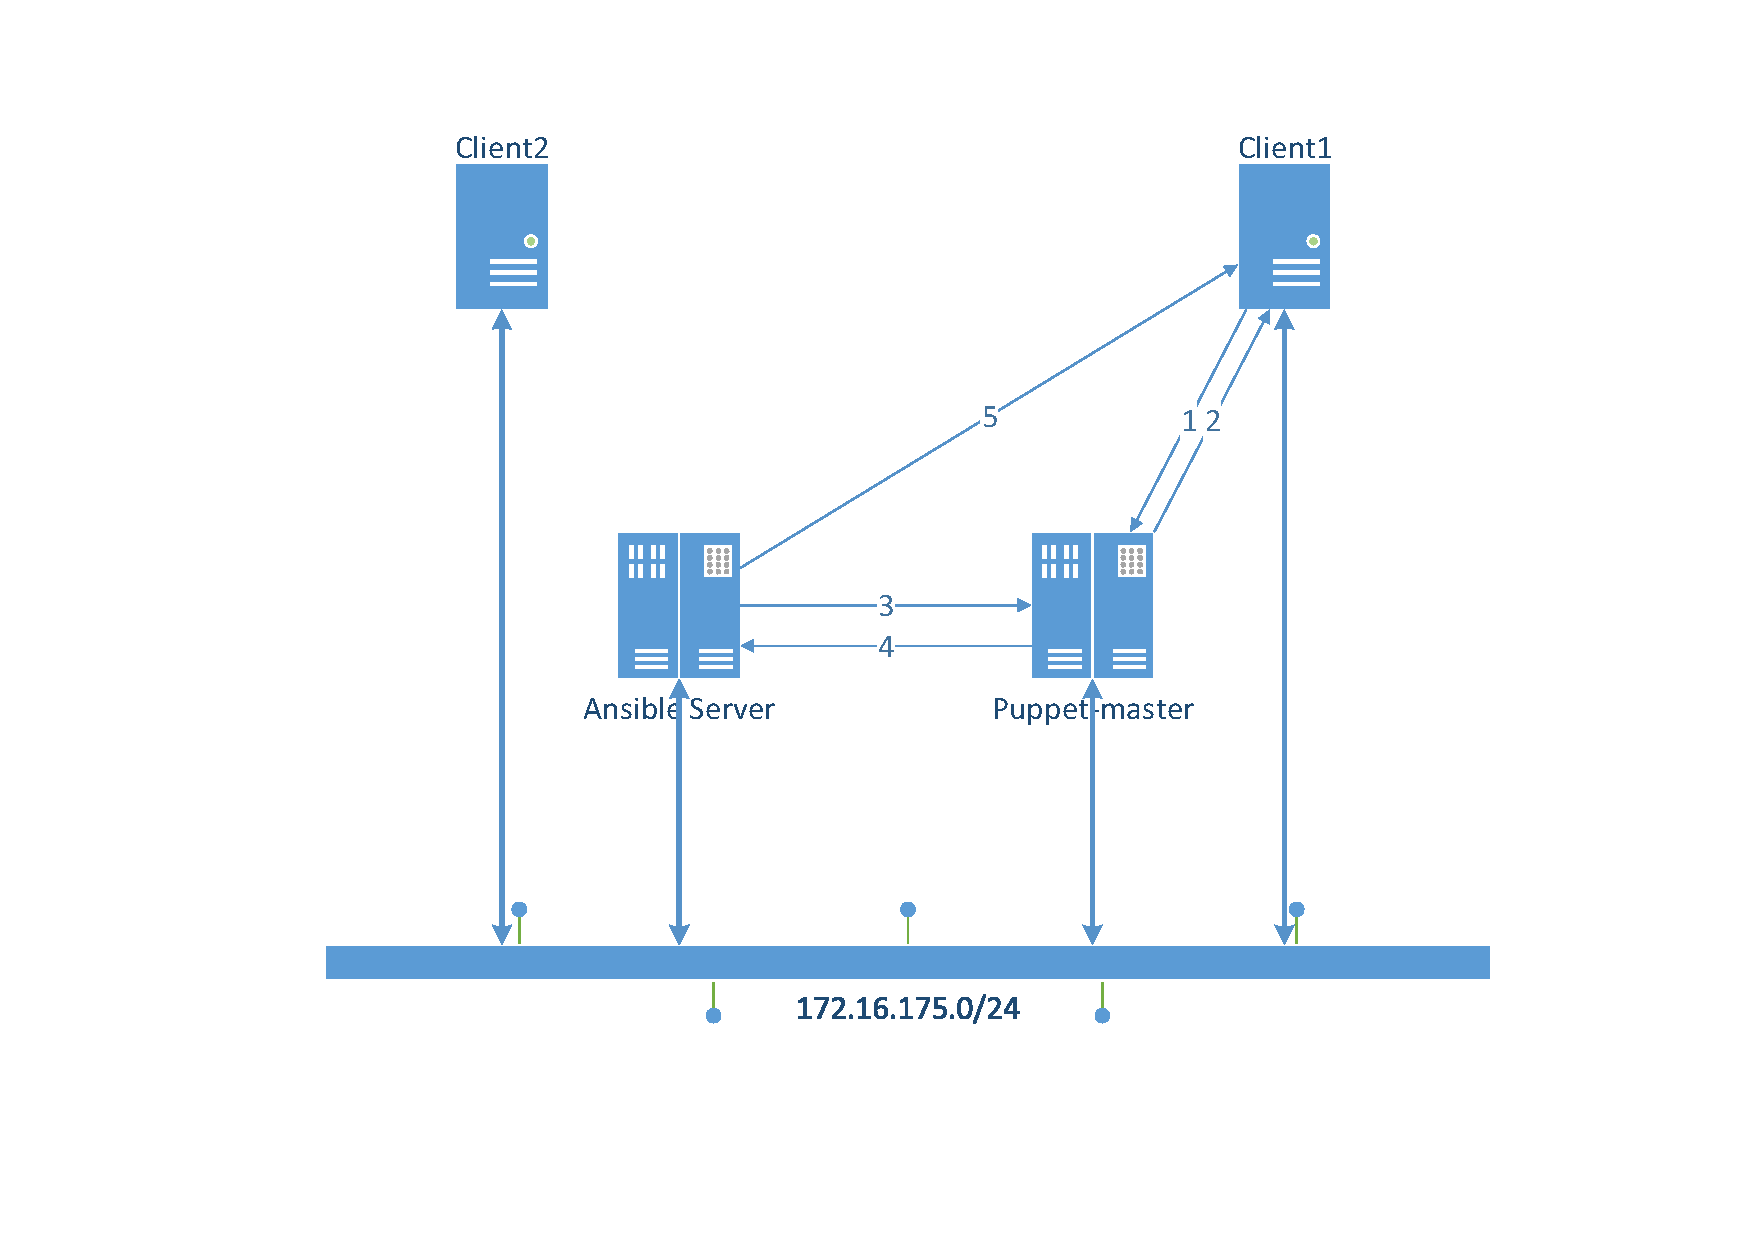
\includegraphics[scale=0.5]{img/PuppettoAnsible.pdf}
        \caption{Migration from Puppet to Ansible.}
        \label{fig:situation1}
\end{figure}

The migration scenario as presented in figure \ref{fig:situation1} shows a method for performing an in-place migration from Puppet to Ansible without affecting end users. The steps below describe how to perform the migration in more detail:

\indent
\begin{itemize}
    \item[\bf Step 1] First, the clients need to be added to Ansible as a group, this should be done by puppet. To make this work. The puppet client needs to be temporary installed on the Ansible server in order to send jobs to this server. Step one in the figure is the installation and first check in of the Puppet client.
    \item[\bf Step 2] Subsequently, the Ansible hosts file need to be updated with the servers from the puppet webservers group. A Puppet job needs to be created for the Puppet clients that tells them to remove the puppet client from the system and allow ssh connections from the Ansible server.
    \item[\bf Step 3/4] Steps three is the client check in and step four is the command set that tells the client to remove itself. This step pulls the puppet-enterprise-uninstaller script from the master. In order to uninstall PE, you must run the uninstaller on each node; you can run it with \texttt{/opt/puppetlabs/bin/puppet-enterprise-uninstaller}. The new playbook (as the set of commands is called within Ansible) is made and tested before changing the management system.
    \item[\bf Step 5/6] When the puppet webservers are added to the Ansible system and the puppet client is removed from the clients the created playbook should be run. For this purpose, a Puppet job is created and steps five and six show the Puppet check in and retrieval of the command set.
    \item[\bf Step 7] Finally, step 7 displays the SSH connection to the client from the Ansible server. This is the end of the client migration from Puppet to Ansible. The puppet-client needs to be removed from the Ansible server when the full migration is completed.
\end{itemize}

One could argue that the full migration can be performed by leveraging Ansible exclusively, as this tool is able to uninstall the Puppet Agent as well by running the uninstaller script. However, we have opted to let Puppet deinstall the Puppet Agent as this is a cleaner method per definition. Additionally, by doing so, we can make sure that no errors occur during the deinstallation phase. If we would use Ansible exclusively, no feedback would be provided if the deinstallation would fail. Besides that, using Ansible for deinstallation would mean a hostile takeover of the system. 

\subsection{Migrating from Ansible to Puppet}\label{subsec:ansibletopuppet}
Although this migration is most likely less frequently performed, it is still valuable in the sense of -for example-  a fallback scenario. As with the previous migration scenario, before Ansible clients can be managed by the Puppet Master there are some prerequisites that need to be satisfied. The packages managed by Ansible need to be reproduced in Puppet and the new clients need to be added to the correct Puppet groups. Otherwise they wont receive the correct packages. When the client checks in at the Puppet Master for the first time, a certificate is exchanged. This should be accepted by default. In order for Puppet to accept all machine certificates an \texttt{autosign.conf} file has to be created in the standard configuration directory \texttt{\$confdir}. The contents of this file function as a whitelist and is very restrictive by default. To accept all certificates, the only contents of this file should be a single wildcard '*'. This means that machines from all possible domains are accepted automatically. Naturally this poses security risks and would require sufficient segregation in a production environment. 

\begin{figure}[!h]
        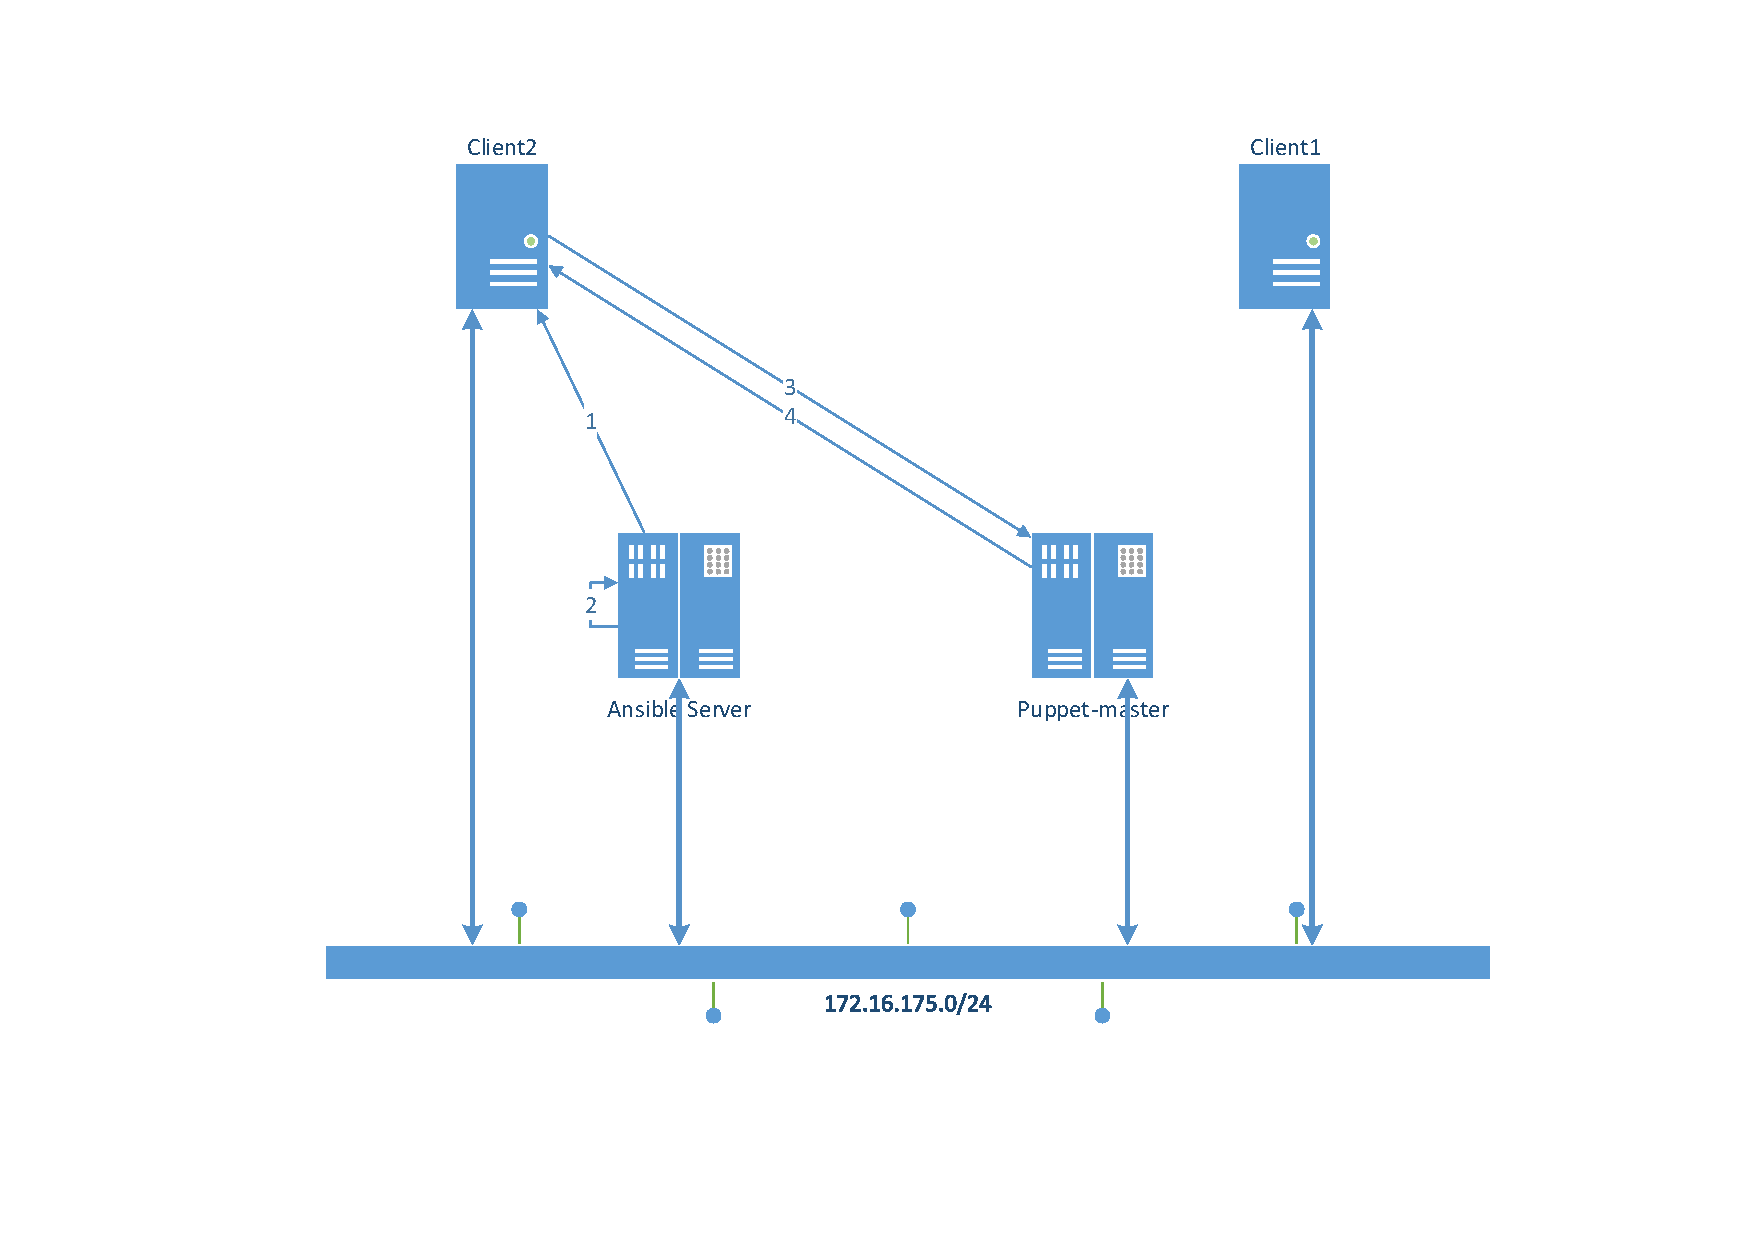
\includegraphics[scale=0.5]{img/AnsibletoPuppet.pdf}
        \caption{Migration from Ansible to Puppet.}
        \label{fig:situation2}
\end{figure}

\indent
\begin{itemize}
    \item[\bf Step 1] Initially an SSH session from Ansible to the Puppet master is initiated to add the machines to the correct groups and prepare the \texttt{autosign.conf} file. All machines managed by Ansible need to receive the Puppet-client in order to be managed by Puppet. This should be done by an Ansible playbook. There are multiple ways to install the Puppet client onto the client group represented in image \ref{fig:situation2} as "Client2". A playbook can be created with the command to install the puppet client using the bash installer provided by the Puppet-master.
    \item[\bf Step 2/3] Step two sends the commands of this playbook to Client2, the playbook is shown in section \ref{app:ansibleplaybook} of the appendixes. An other way is to use the Puppet module within Ansible \cite{ansiblepuppet}. This uses the normal form of a playbook to install the puppet client and the module to configure the puppet client. When the playbook is send to the clients the clients need to be removed from the Ansible hosts file. Therefore the end of the playbook should contain a change into the local Ansible hosts file show in the picture as step three.
    \item[\bf Step 4] Step four shows the first check in from Client2 into Puppet to get the correct version and check in for available jobs.
    \item[\bf Step 5] Step five represents the Puppet Jobs to be transfered to the client. From this moment the system is managed by Puppet instead of Ansible.
\end{itemize}

\subsection{Expectations}\label{subsec:expectations}
For the migration between systems, especially when moving away from a pull based system like Puppet the system needs to be expanded first as explained in the first part of this chapter. The Puppet-client needs to be installed on the Ansible server to make sure the client is added to the host list and the playbook is run in the appropriate time. But there we run into the big disadvantage of Puppet, when using puppet and there are multiple different jobs within one task. You cannot tell what jobs are executed first without special commands. So in order to make this work different jobs need to be prepared and some relations could be created within Puppet. If step one succeeds, proceed to step two, and so on. If step one fail, make a notification and stop the process.  

